% Options for packages loaded elsewhere
\PassOptionsToPackage{unicode}{hyperref}
\PassOptionsToPackage{hyphens}{url}
%


\PassOptionsToPackage{table}{xcolor}

\documentclass[
  10pt,
  letterpaper,
]{article}

\usepackage{amsmath,amssymb}
\usepackage{iftex}
\ifPDFTeX
  \usepackage[T1]{fontenc}
  \usepackage[utf8]{inputenc}
  \usepackage{textcomp} % provide euro and other symbols
\else % if luatex or xetex
  \usepackage{unicode-math}
  \defaultfontfeatures{Scale=MatchLowercase}
  \defaultfontfeatures[\rmfamily]{Ligatures=TeX,Scale=1}
\fi
\usepackage{lmodern}
\ifPDFTeX\else  
    % xetex/luatex font selection
\fi
% Use upquote if available, for straight quotes in verbatim environments
\IfFileExists{upquote.sty}{\usepackage{upquote}}{}
\IfFileExists{microtype.sty}{% use microtype if available
  \usepackage[]{microtype}
  \UseMicrotypeSet[protrusion]{basicmath} % disable protrusion for tt fonts
}{}
\makeatletter
\@ifundefined{KOMAClassName}{% if non-KOMA class
  \IfFileExists{parskip.sty}{%
    \usepackage{parskip}
  }{% else
    \setlength{\parindent}{0pt}
    \setlength{\parskip}{6pt plus 2pt minus 1pt}}
}{% if KOMA class
  \KOMAoptions{parskip=half}}
\makeatother
\usepackage{xcolor}
\usepackage[top=0.85in,left=2.75in,footskip=0.75in]{geometry}
\setlength{\emergencystretch}{3em} % prevent overfull lines
\setcounter{secnumdepth}{-\maxdimen} % remove section numbering

\usepackage{color}
\usepackage{fancyvrb}
\newcommand{\VerbBar}{|}
\newcommand{\VERB}{\Verb[commandchars=\\\{\}]}
\DefineVerbatimEnvironment{Highlighting}{Verbatim}{commandchars=\\\{\}}
% Add ',fontsize=\small' for more characters per line
\usepackage{framed}
\definecolor{shadecolor}{RGB}{241,243,245}
\newenvironment{Shaded}{\begin{snugshade}}{\end{snugshade}}
\newcommand{\AlertTok}[1]{\textcolor[rgb]{0.68,0.00,0.00}{#1}}
\newcommand{\AnnotationTok}[1]{\textcolor[rgb]{0.37,0.37,0.37}{#1}}
\newcommand{\AttributeTok}[1]{\textcolor[rgb]{0.40,0.45,0.13}{#1}}
\newcommand{\BaseNTok}[1]{\textcolor[rgb]{0.68,0.00,0.00}{#1}}
\newcommand{\BuiltInTok}[1]{\textcolor[rgb]{0.00,0.23,0.31}{#1}}
\newcommand{\CharTok}[1]{\textcolor[rgb]{0.13,0.47,0.30}{#1}}
\newcommand{\CommentTok}[1]{\textcolor[rgb]{0.37,0.37,0.37}{#1}}
\newcommand{\CommentVarTok}[1]{\textcolor[rgb]{0.37,0.37,0.37}{\textit{#1}}}
\newcommand{\ConstantTok}[1]{\textcolor[rgb]{0.56,0.35,0.01}{#1}}
\newcommand{\ControlFlowTok}[1]{\textcolor[rgb]{0.00,0.23,0.31}{\textbf{#1}}}
\newcommand{\DataTypeTok}[1]{\textcolor[rgb]{0.68,0.00,0.00}{#1}}
\newcommand{\DecValTok}[1]{\textcolor[rgb]{0.68,0.00,0.00}{#1}}
\newcommand{\DocumentationTok}[1]{\textcolor[rgb]{0.37,0.37,0.37}{\textit{#1}}}
\newcommand{\ErrorTok}[1]{\textcolor[rgb]{0.68,0.00,0.00}{#1}}
\newcommand{\ExtensionTok}[1]{\textcolor[rgb]{0.00,0.23,0.31}{#1}}
\newcommand{\FloatTok}[1]{\textcolor[rgb]{0.68,0.00,0.00}{#1}}
\newcommand{\FunctionTok}[1]{\textcolor[rgb]{0.28,0.35,0.67}{#1}}
\newcommand{\ImportTok}[1]{\textcolor[rgb]{0.00,0.46,0.62}{#1}}
\newcommand{\InformationTok}[1]{\textcolor[rgb]{0.37,0.37,0.37}{#1}}
\newcommand{\KeywordTok}[1]{\textcolor[rgb]{0.00,0.23,0.31}{\textbf{#1}}}
\newcommand{\NormalTok}[1]{\textcolor[rgb]{0.00,0.23,0.31}{#1}}
\newcommand{\OperatorTok}[1]{\textcolor[rgb]{0.37,0.37,0.37}{#1}}
\newcommand{\OtherTok}[1]{\textcolor[rgb]{0.00,0.23,0.31}{#1}}
\newcommand{\PreprocessorTok}[1]{\textcolor[rgb]{0.68,0.00,0.00}{#1}}
\newcommand{\RegionMarkerTok}[1]{\textcolor[rgb]{0.00,0.23,0.31}{#1}}
\newcommand{\SpecialCharTok}[1]{\textcolor[rgb]{0.37,0.37,0.37}{#1}}
\newcommand{\SpecialStringTok}[1]{\textcolor[rgb]{0.13,0.47,0.30}{#1}}
\newcommand{\StringTok}[1]{\textcolor[rgb]{0.13,0.47,0.30}{#1}}
\newcommand{\VariableTok}[1]{\textcolor[rgb]{0.07,0.07,0.07}{#1}}
\newcommand{\VerbatimStringTok}[1]{\textcolor[rgb]{0.13,0.47,0.30}{#1}}
\newcommand{\WarningTok}[1]{\textcolor[rgb]{0.37,0.37,0.37}{\textit{#1}}}

\providecommand{\tightlist}{%
  \setlength{\itemsep}{0pt}\setlength{\parskip}{0pt}}\usepackage{longtable,booktabs,array}
\usepackage{calc} % for calculating minipage widths
% Correct order of tables after \paragraph or \subparagraph
\usepackage{etoolbox}
\makeatletter
\patchcmd\longtable{\par}{\if@noskipsec\mbox{}\fi\par}{}{}
\makeatother
% Allow footnotes in longtable head/foot
\IfFileExists{footnotehyper.sty}{\usepackage{footnotehyper}}{\usepackage{footnote}}
\makesavenoteenv{longtable}
\usepackage{graphicx}
\makeatletter
\def\maxwidth{\ifdim\Gin@nat@width>\linewidth\linewidth\else\Gin@nat@width\fi}
\def\maxheight{\ifdim\Gin@nat@height>\textheight\textheight\else\Gin@nat@height\fi}
\makeatother
% Scale images if necessary, so that they will not overflow the page
% margins by default, and it is still possible to overwrite the defaults
% using explicit options in \includegraphics[width, height, ...]{}
\setkeys{Gin}{width=\maxwidth,height=\maxheight,keepaspectratio}
% Set default figure placement to htbp
\makeatletter
\def\fps@figure{htbp}
\makeatother

% Use adjustwidth environment to exceed column width (see example table in text)
\usepackage{changepage}

% marvosym package for additional characters
\usepackage{marvosym}

% cite package, to clean up citations in the main text. Do not remove.
% Using natbib instead
% \usepackage{cite}

% Use nameref to cite supporting information files (see Supporting Information section for more info)
\usepackage{nameref,hyperref}

% line numbers
\usepackage[right]{lineno}

% ligatures disabled
\usepackage{microtype}
\DisableLigatures[f]{encoding = *, family = * }

% create "+" rule type for thick vertical lines
\newcolumntype{+}{!{\vrule width 2pt}}

% create \thickcline for thick horizontal lines of variable length
\newlength\savedwidth
\newcommand\thickcline[1]{%
  \noalign{\global\savedwidth\arrayrulewidth\global\arrayrulewidth 2pt}%
  \cline{#1}%
  \noalign{\vskip\arrayrulewidth}%
  \noalign{\global\arrayrulewidth\savedwidth}%
}

% \thickhline command for thick horizontal lines that span the table
\newcommand\thickhline{\noalign{\global\savedwidth\arrayrulewidth\global\arrayrulewidth 2pt}%
\hline
\noalign{\global\arrayrulewidth\savedwidth}}

% Text layout
\raggedright
\setlength{\parindent}{0.5cm}
\textwidth 5.25in 
\textheight 8.75in

% Bold the 'Figure #' in the caption and separate it from the title/caption with a period
% Captions will be left justified
\usepackage[aboveskip=1pt,labelfont=bf,labelsep=period,justification=raggedright,singlelinecheck=off]{caption}
\renewcommand{\figurename}{Fig}

% Remove brackets from numbering in List of References
\makeatletter
\renewcommand{\@biblabel}[1]{\quad#1.}
\makeatother

% Header and Footer with logo
\usepackage{lastpage,fancyhdr}
\usepackage{epstopdf}
%\pagestyle{myheadings}
\pagestyle{fancy}
\fancyhf{}
%\setlength{\headheight}{27.023pt}
%\lhead{\includegraphics[width=2.0in]{PLOS-submission.eps}}
\rfoot{\thepage/\pageref{LastPage}}
\renewcommand{\headrulewidth}{0pt}
\renewcommand{\footrule}{\hrule height 2pt \vspace{2mm}}
\fancyheadoffset[L]{2.25in}
\fancyfootoffset[L]{2.25in}
\lfoot{\today}
\makeatletter
\@ifpackageloaded{caption}{}{\usepackage{caption}}
\AtBeginDocument{%
\ifdefined\contentsname
  \renewcommand*\contentsname{Table of contents}
\else
  \newcommand\contentsname{Table of contents}
\fi
\ifdefined\listfigurename
  \renewcommand*\listfigurename{List of Figures}
\else
  \newcommand\listfigurename{List of Figures}
\fi
\ifdefined\listtablename
  \renewcommand*\listtablename{List of Tables}
\else
  \newcommand\listtablename{List of Tables}
\fi
\ifdefined\figurename
  \renewcommand*\figurename{Figure}
\else
  \newcommand\figurename{Figure}
\fi
\ifdefined\tablename
  \renewcommand*\tablename{Table}
\else
  \newcommand\tablename{Table}
\fi
}
\@ifpackageloaded{float}{}{\usepackage{float}}
\floatstyle{ruled}
\@ifundefined{c@chapter}{\newfloat{codelisting}{h}{lop}}{\newfloat{codelisting}{h}{lop}[chapter]}
\floatname{codelisting}{Listing}
\newcommand*\listoflistings{\listof{codelisting}{List of Listings}}
\makeatother
\makeatletter
\makeatother
\makeatletter
\@ifpackageloaded{caption}{}{\usepackage{caption}}
\@ifpackageloaded{subcaption}{}{\usepackage{subcaption}}
\makeatother

\ifLuaTeX
  \usepackage{selnolig}  % disable illegal ligatures
\fi
\usepackage[numbers,square,comma]{natbib}
\bibliographystyle{plos2015}
\usepackage{bookmark}

\IfFileExists{xurl.sty}{\usepackage{xurl}}{} % add URL line breaks if available
\urlstyle{same} % disable monospaced font for URLs
\hypersetup{
  pdftitle={`cpp11armadillo': An `R' Package to Use the Armadillo C++ Library},
  pdfauthor={Mauricio Vargas Sepúlveda; Jonathan Schneider Malamud},
  hidelinks,
  pdfcreator={LaTeX via pandoc}}




\begin{document}
\vspace*{0.2in}

% Title must be 250 characters or less.
\begin{flushleft}
{\Large
\textbf\newline{`cpp11armadillo': An `R' Package to Use the Armadillo
C++
Library} % Please use "sentence case" for title and headings (capitalize only the first word in a title (or heading), the first word in a subtitle (or subheading), and any proper nouns).
}
\newline
\\
% Insert author names, affiliations and corresponding author email (do not include titles, positions, or degrees).
Mauricio Vargas Sepúlveda\textsuperscript{1,2*}, Jonathan Schneider
Malamud\textsuperscript{3}
\\
\bigskip
\textbf{1} Department of Political Science, University of
Toronto, \\ \textbf{2} Munk School of Global Affairs and Public Policy,
University of Toronto, \\ \textbf{3} Department of Electrical and
Computer Engineering, University of Toronto, 
\bigskip

% Insert additional author notes using the symbols described below. Insert symbol callouts after author names as necessary.
% 
% Remove or comment out the author notes below if they aren't used.
%
% Primary Equal Contribution Note
\Yinyang These authors contributed equally to this work.

% Additional Equal Contribution Note
% Also use this double-dagger symbol for special authorship notes, such as senior authorship.
%\ddag These authors also contributed equally to this work.

% Current address notes
\textcurrency Current Address: Dept/Program/Center, Institution Name, City, State, Country % change symbol to "\textcurrency a" if more than one current address note
% \textcurrency b Insert second current address 
% \textcurrency c Insert third current address

% Deceased author note
\dag Deceased

% Group/Consortium Author Note
\textpilcrow Membership list can be found in the Acknowledgments section.

% Use the asterisk to denote corresponding authorship and provide email address in note below.
* 

\end{flushleft}

\section*{Abstract}
``This article introduces `cpp11armadillo', an R package that integrates
the highly efficient Armadillo C++ linear algebra library with R through
the `cpp11' interface. Designed to offer significant performance
improvements for computationally intensive tasks, `cpp11armadillo'
simplifies the process of integrating C++ code into R. This package is
particularly suited for R users requiring efficient matrix operations,
especially in cases where vectorization is not possible. Our benchmark
demonstrate substantial speed gains over native R functions and
Rcpp-based setups.''


\linenumbers

\section{Introduction}\label{introduction}

As R continues to grow in popularity for statistical computing and data
analysis, it can create bottlenecks when working with large datasets.
The need to interface with lower-level languages like C++ to bypass
these bottlenecks has led to the development of tools like `Rcpp'
\citep{eddelbuettel2011}, and more recently, `cpp11' \citep{cpp11}.

`cpp11armadillo' is a novel package that builds upon the existing
Armadillo C++ library \citep{sanderson2016} to provide high-level access
to efficient linear algebra operations directly from R. The existing
`RcppArmadillo' \citep{eddelbuettel2014} already offers this, and
`cpp11armadillo' offers an alternative with modern C++ features, where
we highlight vendoring, that can improve performance and simplify the
its usage.

\section{Features}\label{features}

`cpp11armadillo' simplifies C++ integration by leveraging the `cpp11'
package \citep{cpp11}, which is designed to reduce the complexity of
including C++ code in R. Its core features include:

\begin{itemize}
\item
  High-Performance Matrix Operations: By using Armadillo, cpp11armadillo
  allows users to perform matrix multiplications, inversions, and
  decompositions with minimal overhead. These operations are, for some
  cases, several times faster than their R counterparts.
\item
  Simplified Syntax: Armadillo offers a user-friendly syntax similar to
  that of `MATLAB' \citep{sanderson2016}, making it accessible to R
  users without requiring an extensive background in C++.
\item
  Modern C++ Support: `cpp11armadillo' supports C++11 and newer
  standards, enabling efficient memory management, parallel
  computations, and advanced templates, all integrated into an R
  workflow.
\item
  Integration with R: The package allows direct manipulation of R data
  structures (e.g., vectors, matrices) in C++, providing a seamless
  workflow between the two languages without requiring manual data
  conversion (e.g., such as exporting data to CSV files and continously
  reading them in R to use the C++ output or vice versa).
\end{itemize}

\section{Background}\label{background}

The R programming language was not designed for high-performance
computing, it was created to offer ready-made statistical functions for
the end-user, and its interpreted nature can lead to slow execution
times for computationally intensive tasks \citep{wickham2019, r2024}.
The same applies to Python and other high-level languages.

Compiled languages like C++ offer significant performance improvements
due to their direct access to hardware resources and efficient memory
management. The counterpart is that C++ has a steep learning curve and
it is less user-friendly than R. C++ goals are different, it is designed
to be fast and efficient, and it is not focused on statistical computing
but on general-purpose programming \citep{stroustrup2012}.

However, bottlenecks in R can be solved by using vectorized operations
instead of writing loops, which treats data objects as a whole instead
of element-wise \citep{burns2011}. There are cases where vectorization
is not possible or challenging to implement \citep{burns2011}, and this
is where `cpp11armadillo' comes in and it offers data structures and
functions that are not available in R that facilitate the implementation
of loops and other operations \citep{r2024, sanderson2016}.

Even in spite of these difficulties to work with large datasets or
computationally intensive tasks, R is a growing popularity language for
statistical computing and data analysis, and its community has created
tools to integrate it with SQL databases for memory-efficient data
access \citep{rpostgres}. There are multiple ways to measure a language
popularity, and one of them is the number of R questions in Stack
Overflow, which has been increasing over the years as shown in the
following plot \citep{stackoverflow2024}.

\begin{figure}[H]

{\centering 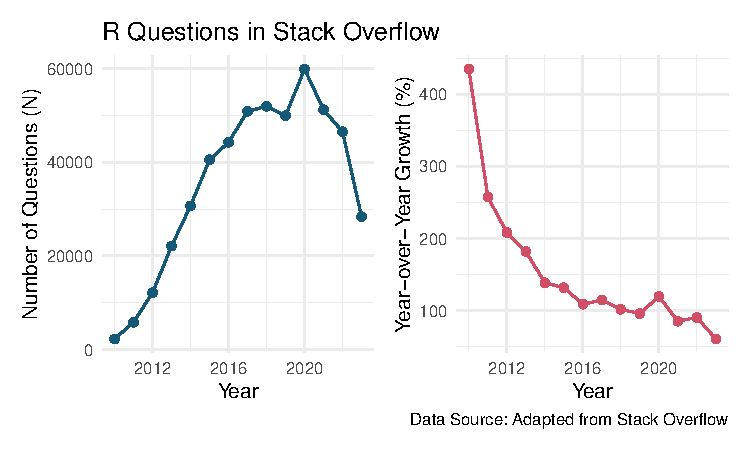
\includegraphics{cpp11armadillo_files/figure-pdf/stackoverflow-1.pdf}

}

\caption{R Questions in Stack Overflow increase from 2,260 in 2010 to
28,385 in 2023 with a peak of 59,895 in 2020.}

\end{figure}%

\section{Modern C++ features}\label{modern-c-features}

`cpp11' is a modern rewrite of the C++ interface for R, designed to
improve safety, performance, and ease of use. It enforces copy-on-write
semantics to prevent unintended modifications to data, ensuring that
changes to objects do not affect other references. Additionally, `cpp11'
provides safer access to R's C API, reducing runtime errors in C++ code.
It also supports ALTREP objects for efficient memory management and
deferred computations, making it ideal for handling large datasets. By
using UTF-8 strings throughout, `cpp11' ensures robust handling of
datasets created in different countries where encodings vary
\citep{cpp11}.

Built on C++11 features like smart pointers and lambdas, `cpp11' offers
a more straightforward and efficient implementation compared to previous
bindings. Its header-only design eliminates ABI compatibility issues,
making it easier to integrate and manage in projects. `cpp11' also
compiles faster, uses less memory, and grows vectors more efficiently,
optimizing performance when dealing with large amounts of data. These
improvements make `cpp11' a powerful, streamlined tool for developers
who need reliable, high-performance C++ bindings for R \citep{cpp11}.

Following from `cpp11', `cpp11armadillo' leverages these modern C++
features to provide a seamless interface between R and the Armadillo
library, offering high-performance linear algebra operations with
minimal overhead. Besides the technical aspects, `cpp11armadillo' offers
vendoring, something not available in `RcppArmadillo', which can
simplify the installation process and reduce dependency issues,
especially when working in environments with restricted access to the
Internet. For instance, the
\href{https://docs.scinet.utoronto.ca/index.php/Niagara_Quickstart}{Niagara
Supercomputer} that we use at the University of Toronto has restricted
access to the Internet, and vendoring can simplify the installation
process.

Vendoring is a well-known concept in the Go community, and it consists
in copying the dependency code directly into a project's source tree.
This approach ensures that dependencies remain fixed and stable,
preventing any external changes from inadvertently breaking the project.
While vendoring offers stability, it comes with trade-offs. The primary
advantage is that updates to the `cpp11armadillo' library will not
disrupt existing code, and it also copies `cpp11' C++ headers. However,
the drawbacks include an increase in package size and the loss of
automatic updates, meaning that bug fixes and new features will only be
available when manually updated.

In other words, vendoring allows the package creator to provide a
dependency-free package that can be installed in any environment without
requiring the end user to install `cpp11' nor `cpp11armadillo'. This
approach makes `cpp11armadillo' a dependency for the developer but not
for the end user.

\section{Usage}\label{usage}

To use `cpp11armadillo', users must first install the package from CRAN
or GitHub. The package includes the Armadillo library, no additional
installation is required. The following code shows how to install the
package:

\begin{Shaded}
\begin{Highlighting}[]
\FunctionTok{install.packages}\NormalTok{(}\StringTok{"cpp11armadillo"}\NormalTok{)}

\CommentTok{\# or}
\NormalTok{remotes}\SpecialCharTok{::}\FunctionTok{install\_github}\NormalTok{(}\StringTok{"pachadotdev/cpp11armadillo"}\NormalTok{)}
\end{Highlighting}
\end{Shaded}

Once installed, users can use the provided package template function to
create a new package that uses C++ code with Armadillo. The package
template includes simple examples and all the necessary files to compile
the code and install the new R package. The following code shows how to
create a new package:

\begin{Shaded}
\begin{Highlighting}[]
\NormalTok{cpp11armadillo}\SpecialCharTok{::}\FunctionTok{create\_package}\NormalTok{(}\StringTok{"cpp11newpackage"}\NormalTok{)}
\end{Highlighting}
\end{Shaded}

The package
\href{https://pacha.dev/cpp11armadillo/index.html}{vignettes} cover the
directories organization and the necessary steps to build an R package
with relatively low setup efforts.

It is important to note that `cpp11armadillo' only work within an R
package, and it is not possible to compile individual C++ scripts on the
fly. This design choice ensures that the R and C++ code is organized
following the organization described in \citet{wickham2023}.

\section{Benchmarks}\label{benchmarks}

In order to evaluate the performance of `cpp11armadillo', we compared it
with native R functions and `RcppArmadillo'. We focused on a single test
consisting in computing the Balassa Index \citep{vargassepulveda2020}.

The R code for the Balassa Index computation is as follows:

\begin{Shaded}
\begin{Highlighting}[]
\NormalTok{balassa\_r }\OtherTok{\textless{}{-}} \ControlFlowTok{function}\NormalTok{(X) \{}
\NormalTok{  B }\OtherTok{\textless{}{-}} \FunctionTok{t}\NormalTok{(}\FunctionTok{t}\NormalTok{(X }\SpecialCharTok{/} \FunctionTok{rowSums}\NormalTok{(X)) }\SpecialCharTok{/}\NormalTok{ (}\FunctionTok{colSums}\NormalTok{(X) }\SpecialCharTok{/} \FunctionTok{sum}\NormalTok{(X)))}
\NormalTok{  B[B }\SpecialCharTok{\textless{}} \DecValTok{1}\NormalTok{] }\OtherTok{\textless{}{-}} \DecValTok{0}
\NormalTok{  B[B }\SpecialCharTok{\textgreater{}=} \DecValTok{1}\NormalTok{] }\OtherTok{\textless{}{-}} \DecValTok{1}
\NormalTok{  B}
\NormalTok{\}}
\end{Highlighting}
\end{Shaded}

The C++ code for the Balassa Index computation from an R matrix is as
follows:

\begin{Shaded}
\begin{Highlighting}[]
\NormalTok{Mat}\OperatorTok{\textless{}}\DataTypeTok{double}\OperatorTok{\textgreater{}}\NormalTok{ balassa\_armadillo}\OperatorTok{(}\AttributeTok{const}\NormalTok{ doubles\_matrix}\OperatorTok{\textless{}\textgreater{}\&}\NormalTok{ x}\OperatorTok{)} \OperatorTok{\{}
\NormalTok{  mat X }\OperatorTok{=}\NormalTok{ as\_Mat}\OperatorTok{(}\NormalTok{x}\OperatorTok{);}
\NormalTok{  mat B }\OperatorTok{=}\NormalTok{ X}\OperatorTok{.}\NormalTok{each\_col}\OperatorTok{()} \OperatorTok{/}\NormalTok{ sum}\OperatorTok{(}\NormalTok{X}\OperatorTok{,} \DecValTok{1}\OperatorTok{);}
\NormalTok{  B }\OperatorTok{=}\NormalTok{ B}\OperatorTok{.}\NormalTok{each\_row}\OperatorTok{()} \OperatorTok{/} \OperatorTok{(}\NormalTok{sum}\OperatorTok{(}\NormalTok{X}\OperatorTok{,} \DecValTok{0}\OperatorTok{)} \OperatorTok{/}\NormalTok{ accu}\OperatorTok{(}\NormalTok{X}\OperatorTok{));}
\NormalTok{  B}\OperatorTok{.}\NormalTok{elem}\OperatorTok{(}\NormalTok{find}\OperatorTok{(}\NormalTok{B }\OperatorTok{\textless{}} \DecValTok{1}\OperatorTok{)).}\NormalTok{zeros}\OperatorTok{();}
\NormalTok{  B}\OperatorTok{.}\NormalTok{elem}\OperatorTok{(}\NormalTok{find}\OperatorTok{(}\NormalTok{B }\OperatorTok{\textgreater{}=} \DecValTok{1}\OperatorTok{)).}\NormalTok{ones}\OperatorTok{();}
  \ControlFlowTok{return}\NormalTok{ B}\OperatorTok{;}
\OperatorTok{\}}
\end{Highlighting}
\end{Shaded}

After implementing the C++ computation in `cpp11armadillo' and
`RcppArmadillo', we compared the execution time of obtaining the Balassa
index year by year for the 2002-2020 period, which involves 19 matrices
with an approximate dimension of \(230 \times 5,100\). After a build
time of 4.4s for `cpp11armadillo' and 9.5s for `RcppArmadillo'. The
following plot reveals almost identical execution times for the
Armadillo function called from `cpp11armadillo' and `RcppArmadillo' with
a marginal advantage for `cpp11armadillo', and both are significantly
faster than the base R function.

\begin{figure}[H]

{\centering 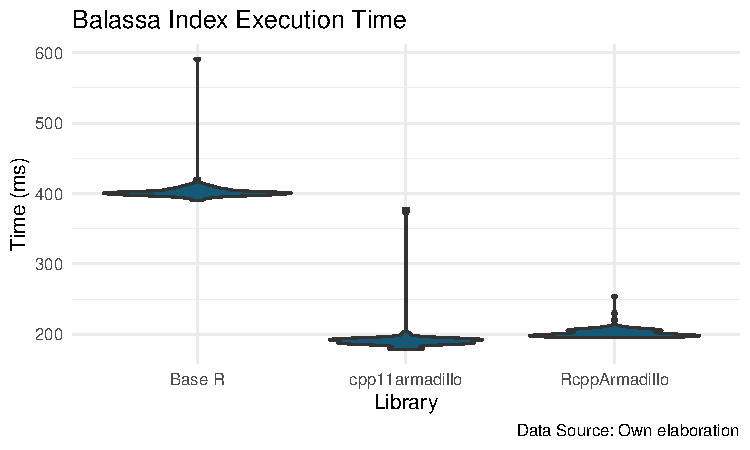
\includegraphics{cpp11armadillo_files/figure-pdf/benchmark-1.pdf}

}

\caption{Balassa Index execution time reveals speed gains of around 50\%
for Armadillo implementations compared to base R.}

\end{figure}%

\newpage

The benchmarks were conducted on a ThinkPad X1 Carbon Gen 9 with the
following specifications:

\begin{itemize}
\tightlist
\item
  Processor: Intel Core i7-1185G7 with eight cores
\item
  Memory: 16 GB LPDDR4Xx-4266
\item
  Operating System: Pop!\_OS 22.04 based on Ubuntu 22.04
\item
  R Version: 4.4.1
\item
  BLAS Library: OpenBLAS 0.3.20
\end{itemize}

\subsection{Conclusion}\label{conclusion}

`cpp11armadillo' provides a simple and efficient way to integrate C++
code with R, leveraging the `cpp11' package and the Armadillo library.
It simplifies the process of writing C++ code for R users, allowing them
to focus on the logic of the algorithm rather than the technical details
of the integration. It can help to solve performance bottlenecks in `R'
code by using the efficient linear algebra operations provided by
Armadillo in cases where vectorization is challenging. `RcppArmadillo'
is a popular package for this purpose, it has existed for nearly a
decade, `cpp11armadillo' offers a different approach with similar
performance.


\nolinenumbers
  \bibliography{references.bib}


\end{document}
